\chapter{Задача построения согласованных моделей декодирования}
\label{ch:pls}

В данной главе приводится формальная постановка задачи декодирования в терминах проекций в скрытое пространство. 
Вводятся понятия скрытого пространства и процедуры согласования образов.
Доказываются теоремы о выборе оптимальной модели декодирования.

%%%%%%%%%%%%%%%%%%%%%%%%%%%%%%%%%%%%%%%%%%%%%%%%
\section{Процесс согласования моделей в пространстве высокой размерности}
\label{sec:ch2:concordance}
%%%%%%%%%%%%%%%%%%%%%%%%%%%%%%%%%%%%%%%%%%%%%%%%

Для постановки задачи декодирования введём предположения о структурах пространств $\bbX$ и $\bbY$.
\begin{assumption}
	Рассмотрим случай, когда пространства $\bbX$ и $\bbY$ имеют избыточную размерность. 
	Это означает, что объекты $\bx$ и $\by$ принадлежат некоторым многообразиям низкой размерности. В простейшем случае такие многообразия могут являться вложениями или линейными подпространствами.
\end{assumption}

\begin{definition}
	Назовём пространство $\bbT \subset \bbR^l$ \textit{скрытым пространством} для пространства $\bbX \subset \bbR^n$ ($l \leq n$), если существуют функция $\bphi_e: \bbX \to \bbT$ и функция $\bphi_d: \bbT  \to \bbX$ такие что
	\[
		\text{для любого } \bx \in \bbX \quad \text{существует } \bt \in \bbT: \bphi_d (\bphi_e(\bx)) = \bphi_d(\bt) = \bx.
	\]
	Функцию $\bphi_e(\bx)$ назовём \textit{функцией кодирования} объекта $\bx$, функцию $\bphi_d(\bt)$  назовём \textit{функцией декодирования}. 
	
	Аналогично введём определение \textit{скрытого пространства}~$\bbU \subset \bbR^s$ для целевого пространства $\bbY$, \textit{функции кодирования} $\bpsi_e: \bbY \to \bbU$ и \textit{декодирования} $\bpsi_d: \bbU  \to \bbY$ такие что
	\[
	 	\text{для любого } \by \in \bbY \quad \text{существует } \bu \in \bbU: \bpsi_d (\bpsi_e(\by)) = \bpsi_d(\bu) = \by.
	\]
\end{definition}

\begin{definition}
	Будем говорить, что скрытые пространства $\bbT$ и $\bbU$ являются \textit{согласованными}, если существует \textit{функция связи} $\bh: \bbT \rightarrow \bbU$, такая что
	\[
		\text{для любого } \bu \in \bbU \quad \text{существует } \bt:  \bu = \bh(\bt).
	\]
\end{definition}

\begin{assumption}
	Предположим, что в задаче прогнозирования~\eqref{ch1:eq:loss_min} пространства $\bbT$ и $\bbU$ являются скрытыми для пространств $\bbX$ и $\bbY$ соответственно. 
	Предположим также, что для данных скрытых пространств $\bbT$ и $\bbU$ существует функция связи~$\bh: \bbT \rightarrow \bbU$. Тогда выполнено
	\[
		\text{для любого } \by \in \bbY \quad \text{существует } \bx \in \bbX: \by = \bpsi_d(\bu) = \bpsi_d(\bh(\bt)) = \bpsi_d(\bh(\bphi_e(\bx))),
	\]
	и общая схема задачи поиска согласованной модели декодирования принимает вид следующей коммутативной диаграммы:
	\begin{equation}
		\begin{tikzpicture}
			\matrix (m) [matrix of math nodes,row sep=3em,column sep=4em,minimum width=2em]
			{
				\bbX \subset \bbR^n & \bbY \subset \bbR^r \\
				\bbT \subset \bbR^\ell & \bbU \subset \bbR^s \\};
			\path[-stealth]
			(m-1-1) edge [black] node [black, above] {$\mathbf{f}$} (m-1-2)
			(m-2-1) edge [black, bend right=10] node [black, right] {$\bphi_d$} (m-1-1)
			(m-2-2) edge [black, bend left=10] node [black, left] {$\bpsi_d$} (m-1-2)
			(m-1-1) edge [black, bend right=10] node [black, left] {$\bphi_e$} (m-2-1)
			(m-1-2) edge [black, bend left=10] node [black, right] {$\bpsi_e$} (m-2-2)
			(m-2-1) edge [black] node [black, above] {$\mathbf{h}$} (m-2-2);
		\end{tikzpicture}
		\label{ch2:eq:decoding_scheme}
	\end{equation}
\end{assumption}

\begin{definition}
	Согласно диаграмме~\eqref{ch2:eq:decoding_scheme}, определим \textit{согласованную} модель декодирования $\mathbf{f}: \bbX \rightarrow \bbY$ как суперпозицию
	\begin{equation}
		\mathbf{f} = \bpsi_d \circ \bh \circ \bphi_e.
		\label{ch2:eq:def_decoding_function}
	\end{equation}
\end{definition}

Таким образом задача прогнозирования~\eqref{ch1:eq:loss_min} сводится к поиску согласованной модели декодирования~\eqref{ch2:eq:def_decoding_function}. 
Для поиска оптимальных параметров функций кодирования $\bphi_e$ и $\bpsi_e$, декодирования $\bphi_d$ и $\bpsi_d$, а также функции связи~$\bh$ ставится задача максимизации $\textit{функции согласования проекций}$
\[
	g: \bbT \times \bbU \rightarrow \bbR, \quad g(\bT, \bU) = g(\bphi_e(\bX), \bpsi_e(\bY)) \rightarrow \max_{\bphi_e, \bpsi_e, \bh}.
\]

Сформулируем примеры методов снижения размерности пространства, описанные в разделе~\ref{sec:ch1:dim_reduction}, в терминах задачи построения согласованной модели декодирования.

\textbf{Метод главных компонент.} 
Метод главных компонент снижает размерность исходных данных и сохраняет максимальную дисперсию между полученными проекциями. 
Линейная модель PCA представляет собой ортогональное линейное преобразование исходного признакового пространства в скрытое пространство меньшей размерности. 
Базисные вектора в скрытом пространстве строятся так, чтобы выборочная дисперсия столбцов проекций матрицы~$\bX$ была максимальной:
\begin{equation*}
	\bp = \argmax_{\|\bp\|_{2} = 1} [\text{var}(\bX \textbf{p})].
\end{equation*}

Функции кодирования $\bphi_e: \bbR^m \to \bbR^l$ и декодирования $\bphi_d: \bbR^l \to \bbR^m$ имеют вид
\begin{equation*}
	\bphi_e(\bX) =  \underset{n \times m}\bX \cdot \underset{m \times l}\bP^{\T}, \quad	\bphi_d(\bT) =  \underset{n \times l}\bT \cdot \underset{l \times m}\bP,
	\label{ch2:eq:PCA2}
\end{equation*}
где $\bP = [\bp_1, \dots, \bp_l].$ Здесь матрица $\bP$ является ортогональной матрицей, то есть $\bP^{-1} = \bP^{\T}$.
Метод PCA не согласует исходные переменные и целевые переменные. 
А именно алгоритм PCA не находит функции кодирования $\bpsi_e$ и декодирования $\bpsi_d$, а также функцию связи $\bh$. 
Из-за этого зависимости в обоих пространствах не учитываются.
Пример некорректной работы  метода в случае наличия зависимостей как в исходном, так и в целевом пространстве, показан в разделе~\ref{sec:ch1:dim_reduction}.

\textbf{Метод наименьших частичных квадратов.}
В методе PLS  функции кодирования и декодирования имеют вид
\begin{align*}
	\bphi_e(\bX) &= \bX \bW, \quad \bpsi_e(\bY) = \bY \bC, \\
	\bphi_d(\bT) &= \bT \bP^{\T}, \quad \bpsi_d(\bU) = \bU \bQ^{\T}.
\end{align*}
Функция связи $\bh$ имеет вид линейной модели, связывающей образы проекций в скрытом пространстве $\bu = \bh(\bt) = \bB^{\T} \bt$.
В данном случае схема декодирования~\eqref{ch2:eq:decoding_scheme} принимает вид следующей коммутативной диаграммы.
\begin{equation*}
	\begin{tikzpicture}
		\matrix (m) [matrix of math nodes,row sep=3em,column sep=4em,minimum width=2em]
		{
			\bbX \subset \bbR^n & \bbY \subset \bbR^r \\
			\bbT \subset \bbR^\ell & \bbU \subset \bbR^s \\};
		\path[-stealth]
		(m-1-1) edge [black] node [black, above] {$\mathbf{f}$} (m-1-2)
		(m-1-1) edge [black, bend right=10] node [black, left] {$\bW$} (m-2-1)
		(m-2-1) edge [black, bend right=10] node [black, right] {$\bP$} (m-1-1)
		(m-1-2) edge [black, bend left=10] node [black, right] {$\bC$} (m-2-2)
		(m-2-2) edge [black, bend left=10] node [black, left] {$\bQ$} (m-1-2)
		(m-2-1) edge [black] node [black, above] {$\bB$} (m-2-2);
	\end{tikzpicture}
\end{equation*}
В разделе~\ref{sec:ch2:pls_proof} приводится подробная процедура нахождения оптимальных матриц $\bP$, $\bQ$, $\bW$, $\bC$, $\bB$ с доказательством корректности.

\textbf{Канонический анализ корреляций.} Канонический анализ корреляций находит два набора базисных векторов $\{\bw_{\bx_i}\}_{i=1}^{l}$, $\bw_{\bx} \in \mathbb{R}^{m}$, и $\{\bw_{\by_i}\}_{i=1}^{l}, \; \bw_{\by} \in \mathbb{R}^{k}$, один для матрицы $\bX$, другой для матрицы $\bY$, так чтобы коэффициент корреляции между проекциями переменных на эти базисные векторы был максимальным. Функция согласования для CCA имеет вид
\begin{equation*}
	g(\bX \bW_{\bx}, \bY \bW_{\by}) = \text{corr}(\bX \bW_{\bx}, \bY \bW_{\by}),
\end{equation*}
\noindent где $\text{corr}(\bX \bw_{\bx}, \bY \bw_{\by})$~-- коэффициент корреляции между векторами.

Таким образом, функции кодирования имеют вид
\begin{equation*}
	\bphi_e(\bX) = \bX \bW_{\bx} , \;\;
	\bpsi_e(\bY) = \bY \bW_{\by},
\end{equation*}
где первые столбцы матриц весов находятся как векторы, максимизирующие функцию согласования $g$. Далее ищутся векторы, максимизирующие $g$, но с ограничением, ортогональности первой парой векторов. Процедура продолжается до тех пор, пока число векторов не станет равным $l$.

\textbf{Нелинейный канонический анализ корреляций.}
Помимо линейных моделей декодирования рассматриваются нелинейные методы. 
В данном случае функции кодирования и декодирования являются нелинейными нейросетями вида
\begin{align*}
	\bT &= \bphi_e(\bX) =  \bW_\bx^L \sigma(\dots \sigma(\bW_\bx^2 \sigma(\bX \bW_\bx^1)) \dots ), \\
	\bU &= \bpsi_e(\bY) =  \bW_\by^L \sigma(\dots \sigma(\bW_\by^2 \sigma(\bY \bW_\by^1)) \dots ), \\
	\bX &= \bphi_d(\bT) =  \bW_\bt^L \sigma(\dots \sigma(\bW_\bt^2 \sigma(\bT \bW_\bt^1)) \dots ), \\
	\bY &= \bpsi_d(\bU) =  \bW_\bu^L \sigma(\dots \sigma(\bW_\bu^2 \sigma(\bU \bW_\bu^1)) \dots ).
\end{align*}
Каждая нейросеть является суперпозицией последовательных умножений на матрицы параметров и применения поэлементных функций активаций.

Требуется найти такие параметры, при которых функция согласования~$g$ достигает своего максимума:
\begin{equation}
	g(\bT, \bU) \rightarrow \max_{\bW},
	\label{ch2:eq:concordance}
\end{equation}
где $\bW = \bigl\{\bW_\bx^i, \bW_\by^i, \bW_\bt^i, \bW_\bu^i\bigr\}_{i=1}^L$.

Процесс согласования заключается в максимизации функции согласования $g(\bt, \bu)$ по параметрам нейросетей.
В работе~\cite{andrew2013deep} рассматривается частный случай задачи~\eqref{ch2:eq:concordance}. 
При использовании в качестве функции согласования корреляции между проекциями $g(\bt, \bu) = \textnormal{corr}(\bt, \bu)$ частная производная функции согласования по первому аргументу принимает вид
\[
	\frac{\partial g(\bt, \bu)}{\partial \bt} = \frac{1}{\ell - 1} \left(\bSigma_1^{-1/2} \bU \bV^{\T} \bSigma_2^{-1/2} \bU - \bSigma_1^{-1/2} \bU \bD \bV^{\T} \bSigma_1^{-1/2} \right),
\]
где $\bU, \bD, \bV = \textnormal{SVD}(\bSigma)$, \, $\bSigma = \bSigma_1^{-1/2} \bSigma_{12} \bSigma_2^{-1/2} $, \, $\bSigma_1 = \frac{1}{\ell - 1} \bT \bT^{\T}$, \, $\bSigma_2 = \frac{1}{\ell - 1} \bU \bU^{\T}$, \, $\bSigma_{12} = \frac{1}{\ell - 1} \bT \bU^{\T}$.
Аналогичное выражение имеет частная производная по второму аргументу.
Полученное выражение для градиента позволяет построить эффективный алгоритм для решения задачи с использованием градиентных методов оптимизации.

%%%%%%%%%%%%%%%%%%%%%%%%%%%%%%%%%%%%%%%%%%%%%%%%
\section{Доказательство корректности работы алгоритмов PLS и CCA}
\label{sec:ch2:pls_proof}
%%%%%%%%%%%%%%%%%%%%%%%%%%%%%%%%%%%%%%%%%%%%%%%%

Псевдокод метода регрессии PLS приведен в алгоритме~\ref{ch2:pls_pseudocode}.
Алгоритм итеративно на каждом из $l$ шагов вычисляет по одному столбцу $\bt_k$, $\bu_k$, $\bp_k$, $\bq_k$ матриц $\bT$, $\bU$, $\bP$, $\bQ$ соответственно. 
После вычисления следующего набора векторов из матриц $\bX$, $\bY$ вычитаются очередные одноранговые аппроксимации. 
При этом предполагается, что исходные матрицы~$\bX$ и~$\bY$ нормированы (имеют нулевое среднее и единичное среднее отклонение).

\begin{algorithm}[h]
	\caption{Алгоритм PLS}
	\label{ch2:pls_pseudocode}
	\begin{algorithmic}[1]
		\REQUIRE $\bX, \bY, l$;
		\ENSURE $\bT, \bP, \bQ$;
		\STATE нормировать матрицы $\bX$ и $\bY$ по столбцам
		\STATE инициализировать $\bu_0$ (первый столбец матрицы $\bY$)
		\STATE $\bX_1 = \bX; \bY_1 = \bY$
		\FOR{$k=1,\dots, l$}
		\REPEAT
		\vspace{0.1cm}
		\STATE $\bw_k := \bX_k^{\T} \bu_{k-1} / (\bu_{k-1}^{\T} \bu_{k-1}); \quad \bw_k: = \frac{\bw_k}{\| \bw_k \|}$
		\vspace{0.1cm}
		\STATE $\bt_k := \bX_k \bw_k$
		\vspace{0.1cm}
		\STATE $\bc_k := \bY_k^{\T} \bt_k / (\bt_k^{\T} \bt_k); \quad \bc_k: = \frac{\bc_k}{\| \bc_k \|}$
		\vspace{0.1cm}
		\STATE $\bu_k := \bY_k \bc_k$
		\UNTIL{$\bt_k$ не стабилизируется}
		\vspace{0.1cm}
		\STATE $\bp_k:= \bX_k^{\T}\bt_k/(\bt_k^{\T}\bt_k),\ 
		\bq_k := \bY_k^{\T}\bt_k/(\bt_k^{\T}\bt_k)$
		\vspace{0.2cm}
		\STATE $\bX_{k+1} :=  \bX_k - \bt_k \bp_k^{\T}$
		\vspace{0.2cm}
		\STATE $\bY_{k + 1} :=  \bY_k - \bt_k \bq_k^{\T}$ 
		\ENDFOR
	\end{algorithmic}
\end{algorithm}

Вектора $\bt_k$ и $\bu_k$ из внутреннего цикла aлгоритма~\ref{ch2:pls_pseudocode}
содержат информацию о матрице исходных объектов $\bX$ и матрице целевых объектов $\bY$ соответственно. 
Блоки из шагов (6)--(7) и шагов (8)--(9)~--- аналоги алгоритма PCA для матриц $\bX$ и $\bY$~\cite{geladi1988pls}. 
Последовательное выполнение блоков позволяет учесть взаимную связь между матрицами $\bX$ и $\bY$.

Теоретическое обоснование алгоритма PLS следует из следующих утверждений.
\begin{statement}
	Максимизации ковариации между векторами $\bt_k$ и $\bu_k$ сохраняет дисперсию столбцов матриц~$\bX$ и~$\bY$ и учитывает их линейную зависимость.
\end{statement}
\begin{proof}
	Утверждение следует из равенства
	\[
	\text{cov} (\bt_k, \bu_k) = \text{corr} (\bt_k, \bu_k) \cdot \sqrt{\text{var}(\bt_k)} \cdot \sqrt{\text{var}(\bu_k)}.
	\]
	Максимизация дисперсий векторов $\bt_k$ и $\bu_k$ отвечает за сохранение информации об исходных матрицах, 
	корреляция между векторами отвечает взаимосвязи между $\bX$ и~$\bY$. 
\end{proof}

Во внутреннем цикле aлгоритма~\ref{ch2:pls_pseudocode} вычисляются нормированные вектора весов $\bw_k$ и $\bc_k$. 
Из данных векторов строятся матрицы весов $\bW$ и $\bC$ соответственно.

\begin{statement}
	В результате выполнения внутреннего цикла вектора $\bw_k$ и $\bc_k$ будут собственными векторами матриц $\bX_k^{\T} \bY_k \bY_k^{\T} \bX_k$ и $\bY_k^{\T} \bX_k \bX_k^{\T} \bY_k$, соответствующими максимальным собственным значениям.
	
	\begin{equation*}
		\bw_k \varpropto \bX_k^{\T} \bu_{k-1} \varpropto \bX_k^{\T} \bY_k \bc_{k-1} \varpropto \bX_k^{\T} \bY_k \bY_k^{\T} \bt_{k-1} \varpropto \bX_k^{\T} \bY_k \bY_k^{\T} \bX_k \bw_{k-1},
	\end{equation*}
	\begin{equation*}
		\bc_k \varpropto \bY_k^{\T} \bt_k \varpropto \bY_k^{\T} \bX_k \bw_k \varpropto \bY_k^{\T} \bX_k \bX_k^{\T} \bu_{k-1} \varpropto \bY_k^{\T} \bX_k \bX_k^{\T} \bY_k \bc_{k-1},
	\end{equation*}
	где символ $\varpropto$ означает равенство с точностью до мультипликативной константы. 
	\label{ch2:stat:eig}
\end{statement}
\begin{proof}
	Утверждение следует из того факта, что правила обновления векторов $\bw_k$, $\bc_k$ совпадают с итерацией алгоритма поиска максимального собственного значения. 
	Данный алгоритм основан на следующем факте.
	Если матрица $\mathbf{A}$ диагонализуема, $\bx$~--- некоторый вектор, то
	
	\[
	\lim_{k \rightarrow \infty} \mathbf{A}^k \bx = \lambda_{\max}(\mathbf{A}) \cdot \mathbf{v}_{\max},
	\]
	где $ \lambda_{\max} (\mathbf{A})$~--- максимальное собственное значение матрицы $\mathbf{A}$, $\mathbf{v}_{\max}$~---собственный вектор матрицы $\mathbf{A}$, соответствующий~$\lambda_{\max} (\mathbf{A})$.
	
\end{proof}

\begin{statement}
	Обновление векторов по шагам (6)--(9) aлгоритма~\ref{ch2:pls_pseudocode} соответствует максимизации ковариации между векторами~$\bt_k$ и~$\bu_k$.
\end{statement}
\begin{proof}
	Максимальная ковариация между векторами~$\bt_k$ и~$\bu_k$ равна максимальному собственному значению матрицы~$\bX_k^{\T} \bY_k \bY_k^{\T} \bX_k$:
	\begin{align*}
		\max_{\bt_k, \bu_k}  \text{cov} (\bt_k, \bu_k)^2 &= \max_{\substack{\|\bw_k\|=1 \\ \|\bc_k\| = 1}} \text{cov} \left( \bX_k \bw_k, \bY_k \bc_k \right)^2 = \max_{\substack{\|\bw_k\|=1 \\ \|\bc_k\| = 1}} \text{cov} \left(\bc_k^{\T}  \bY_k^{\T} \bX_k \bw_k \right)^2 = \\
		&= \max_{\|\bw_k\| = 1} \text{cov} \left\|\bY_k^{\T} \bX_k \bw_k \right\|^2 = \max_{\|\bw_k\| = 1} \bw_k^{\T} \bX_k^{\T} \bY_k \bY_k^{\T} \bX_k \bw_k = \\
		& = \lambda_{\max} \left( \bX_k^{\T} \bY_k \bY_k^{\T} \bX_k \right),
s	\end{align*}
	где~$\lambda_{\max} (\mathbf{A})$~--- максимальное собственное значение матрицы $\mathbf{A}$.
	Применяя утверждение~\ref{ch2:stat:eig}, получаем требуемое.
\end{proof}

После завершения внутреннего цикла на шаге (11) вычисляются вектора $\bp_k$, $\bq_k$ проецированием столбцов матриц $\bX_k$ и $\bY_k$ на вектор $\bt_k$. 
Для перехода на следующий шаг необходимо вычесть из матриц $\bX_k$ и $\bY_k$ одноранговые аппроксимации $\bt_k \bp_k^{\T}$ и $\bt_k \bq_k^{\T}$
\begin{align*}
	\bX_{k + 1} &= \bX_{k} - \bt_k \bp_k^{\T} = \bX - \sum_k \bt_k \bp_k^{\T}, \\
	\bY_{k + 1} &= \bY_{k} - \bt_k \bq_k^{\T} = \bY - \sum_k \bt_k \bq_k^{\T}.
\end{align*}
При этом каждый следующий вектор~$\bt_k$ оказывается ортогонален всем векторам~$\bt_i$, $i=1, \dots, k$.

Для получения прогнозов модели и нахождения параметров модели 
домножим справа формулу~\eqref{ch1:eq:PLS_X} на матрицу $\bW$. Строки матрицы невязок $\bE$ ортогональны столбцам матрицы $\bW$, поэтому 
\[
\bX \bW = \bT \bP^{\T} \bW.
\] 

Линейное преобразование между объектами в исходном и латентном пространстве имеет вид
\begin{equation}
	\bT = \bX \bW^*,
	\label{ch2:eq:W*}
\end{equation}
где $\bW^* = \bW (\bP^{\T} \bW)^{-1}$. 

Матрица параметров модели~\ref{ch1:eq:lin_reg_model} находится из уравнений~\eqref{ch1:eq:PLS_Y},~\eqref{ch2:eq:W*}
\begin{equation}
	\bY = \bT \bQ^{\T} + \bE = \bX \bW^* \bQ^{\T} + \bE = \bX \bTheta + \bE.
	\label{ch2:eq:pls_model}
\end{equation}
Таким образом, параметры модели~\eqref{ch1:eq:lin_reg_model} равны
\begin{equation*}
	\bTheta = \bW (\bP^{\T} \bW)^{-1} \bQ^{\T}.
\end{equation*}

Финальная модель~\eqref{ch2:eq:pls_model} является линейной, низкоразмерной в скрытом пространстве. 
Это снижает избыточность данных и повышает стабильность модели.

%%%%%%%%%%%%%%%%%%%%%%%%%%%%%%%%%%%%%%%%%%%%%%%%
\section{Аддитивная суперпозиция моделей декодирования}
\label{sec:ch2:superposition}
%%%%%%%%%%%%%%%%%%%%%%%%%%%%%%%%%%%%%%%%%%%%%%%%

Пусть $\mathbf{f}_1(\bx_1, \bTheta_1)$, $\mathbf{f}_2(\bx_2, \bTheta_2)$ -- линейные модели декодирования сигналов. 
Рассмотрим аддитивную суперпозицию моделей декодирования, то есть модель~\eqref{ch1:eq:reg_model} вида
\begin{equation}
	\by = \mathbf{f}(\bx, \bTheta) + \bepsilon = \bTheta_1 \bx_1 + \bTheta_2 \bx_2 + \bepsilon,
	\label{ch2:eq:two_modal_reg_model}
\end{equation}
где объект $\bx = [\bx_1, \bx_2] \in \bbR^n$ состоит из двух подвекторов $\bx_1 \in \bbR^k$, $\bx_2 \in \bbR^{n - k}$. Тем самым матрица параметров $\bTheta \in \bbR^{n \times r}$ состоит из двух подматриц $\bTheta_1 \in \bbR^{k \times r}$, $\bTheta_2 \in \bbR^{n - k \times r}$. 

\begin{statement}
	\label{ch2:stat:two_modal_params}
	Матрица параметров $\bTheta$ для модели~\eqref{ch2:eq:two_modal_reg_model}, доставляющая минимум функции ошибки~\eqref{ch1:eq:l2_loss_function}, имеет вид:
	\begin{align*}
		\bTheta_1 &= (\bX_1^{\T} \bM_{\bX_2} \bX_1)^{-1} \bX_1^{\T} \bM_{\bX_2} \bY, \\
		\bTheta_2 &= (\bX_2^{\T} \bM_{\bX_1} \bX_2)^{-1} \bX_2^{\T} \bM_{\bX_1} \bY,
	\end{align*}
	где $\bM_{\bX_1} = (\bI - \bP_{\bX_1})$, $\bM_{\bX_2} = (\bI - \bP_{\bX_2})$, $\bP_{\bX_1} = \bX_1 (\bX_1^{\T} \bX_1)^{-1} \bX_1^{\T}$, $\bP_{\bX_2} = \bX_2 (\bX_2^{\T} \bX_2)^{-1} \bX_2^{\T}$.
\end{statement}

\begin{proof}
	Домножим уравнение $\bY = \bX \bTheta$ слева на матрицу $\bX{\T}$
	\[
		\bX^{\T} \bX \bTheta = \bX^{\T} \bY; \quad \Rightarrow \quad
		\begin{cases*}
			\bX_1^{\T} \bX_1 \bTheta_1 + \bX_1^{\T} \bX_2 \bTheta_2 = \bX_1^{\T} \bY \\
			\bX_2^{\T} \bX_1 \bTheta_1 + \bX_2^{\T} \bX_2 \bTheta_2 = \bX_2^{\T} \bY 
		\end{cases*}
	\]
	Выразим из этой системы параметры каждой отдельной модели в суперпозиции:
	\[
		\begin{cases}
			\bTheta_1 = (\bX_1^{\T} \bX_1)^{-1} \bX_1^{\T} (\bY - \bX_2 \bTheta_2) \\
			\bTheta_2 = (\bX_2^{\T} \bX_2 )^{-1}  \bX_2^{\T} (\bY - \bX_1 \bTheta_1)
		\end{cases}
	\]
	Подставим полученные выражения для $\bTheta_1$ и $\bTheta_2$ в исходную систему:
	\[
				\begin{cases*}
					\bX_1^{\T} \bP_{\bX_1} (\bY - \bX_2 \bTheta_2) + \bX_1^{\T} \bX_2 \bTheta_2 = \bX_1^{\T} \bY \\
					\bX_2^{\T} \bX_1 \bTheta_1 + \bX_2^{\T}\bP_{\bX_2} (\bY - \bX_1 \bTheta_1) = \bX_2^{\T} \bY 
				\end{cases*}
	\]
	Выразив матрицы параметров, получим требуемые выражения.
\end{proof}

Заметим, что матрицы $\bP_{\bX_1}$ и $\bP_{\bX_2}$ являются матрицами проекций на подпространства, образованные линейными оболочками столбцов матриц $\bX_1$ и $\bX_2$ соответственно.
Таким образом матрицы $\bM_{\bX_1}$ и $\bM_{\bX_2}$ являются матрицами проекций на ортогональные подпространства.

\begin{statement}
	\label{ch2:stat:two_modal_theta2}
	Оптимальная подматрица $\bTheta_2$ в модели~\eqref{ch2:eq:two_modal_reg_model} является решением задачи регрессии
	\begin{equation}
		\| \bY_1 -  \bX_{21} \bTheta_2 \| \rightarrow \min_{\bTheta_2},
		\label{ch2:eq:two_modal_fwl}
	\end{equation}
	где $\bY_1 = \bM_{\bX_1} \bY$, $\bX_{21} = \bM_{\bX_1} \bX_2$.
\end{statement}

\begin{proof}
	Матрица $\bM_{\bX_1}$ является матрицей проекции на ортогональное подпространство, построенное на линейной оболочке столбцов матрицы $\bX_1$. Таким образом, матрица $\bM_{\bX_1}$ является идемпотентной ($\bM_{\bX_1}{\T} \bM_{\bX_1} = \bM_{\bX_1}$). 
	Таким образом, используя утверждение~\ref{ch2:stat:two_modal_params},
	\begin{multline*}
		\bTheta_2 = (\bX_2^{\T} \bM_{\bX_1} \bX_2)^{-1} \bX_2^{\T} \bM_{\bX_1} \bY = (\bX_2^{\T} \bM_{\bX_1}^{\T} \bM_{\bX_1} \bX_2)^{-1} \bX_2^{\T} \bM_{\bX_1}^{\T} \bM_{\bX_1} \bY = \\
		= ((\bM_{\bX_1} \bX_2)^{\T} (\bM_{\bX_1} \bX_2)^{\T})^{-1} (\bM_{\bX_1} \bX_2)^{\T} (\bM_{\bX_1} \bY) = (\bX_{21}^{\T} \bX_{21})^{-1} \bX_{21}^{\T} \bY_1.
	\end{multline*}
	Согласно теореме Гаусса-Маркова $\bTheta_2$ является решением задачи регрессии~\eqref{ch2:eq:two_modal_fwl}.
\end{proof}

Таким образом для нахождении оптимальной модели декодирования $\mathbf{f}(\bx_2, \bTheta_2)$ необходимо спроецировать матрицы $\bY$ и $\bX_2$ на подпространства, ортогональные подпространству, образованному линейной оболочкой столбцов матрицы $\bX_1$.

Похожие результаты были доказаны в эконометрике в работах~\cite{frisch1933partial,lovell1963seasonal,cinelli2020making}. Аналогичное утверждение верно и для матрицы~$\bTheta_1$. 

\begin{statement}
	Если в задаче~\eqref{ch2:eq:two_modal_reg_model} $\text{span}(\bX_1) \cap \text{ span}(\bX_2) = \emptyset$, то есть столбцы матрицы $\bX_1$ ортогональны столбцам матрицы~$\bX_2$, то $\bTheta_2$ является решением задачи регрессии
	\[
		\| \bY -  \bX_{2} \bTheta_2 \| \rightarrow \min_{\bTheta_2}.
	\]
\end{statement}

\begin{proof}
	Используя факт, что $\bI = \bP_{\bX_1} + \bM_{\bX_1}$ и $\bX_2 \bX_1 = 0$, получаем
	\begin{multline*}
		(\bX_2^{\T} \bX_2)^{-1} \bX_2^{\T} \bY = (\bX_2^{\T} \bX_2)^{-1} \bX_2^{\T} (\bP_{\bX_1} + \bM_{\bX_1}) \bY = \\ = (\bX_2^{\T} \bX_2)^{-1} \bX_2^{\T} \bM_{\bX_1} \bY  = (\bX_{21}^{\T} \bX_{21})^{-1} \bX_{21}^{\T} \bY_1
	\end{multline*}
	Используя утверждение~\ref{ch2:stat:two_modal_theta2}, получаем требуемое утверждение.
\end{proof}
Данное утверждение показывает, что в случае независимых столбцов матриц $\bX_1$ и $\bX_2$ задача регрессии для аддитивной суперпозиции моделей~\eqref{ch2:eq:two_modal_reg_model} распадается на две независимые подзадачи.

Из выше доказанных утверждений прямо следует следующая теорема.

\begin{theorem}
	Если в задаче~\eqref{ch2:eq:two_modal_reg_model} $\text{span}(\bX_1) \neq \text{ span}(\bX_2)$, то ошибка аддитивной суперпозиции моделей не превышает ошибки каждой из отдельных моделей
	\begin{align*}
		\mathcal{L}(\bTheta^*, \bX, \bY) &\leq \mathcal{L}(\bTheta_1, \bX_1, \bY), \\
		\mathcal{L}(\bTheta^*, \bX, \bY) &\leq \mathcal{L}(\bTheta_2, \bX_2, \bY).
	\end{align*}
\end{theorem}

Рассмотрим случай линейной авторегрессионной модели $\mathbf{f}_{\text{AR}}^y$ и линейной регрессионной модели $\mathbf{f}_{\text{R}}^{xy}$. 
Пусть предсказательная модель $\mathbf{f}^{xy}: \bbR^{h_x \times m} \times \bbR^{h_y \times r} \rightarrow \bbR^{p \times r}$ является аддитивной суперпозицией авторегрессионной и регрессионной моделей.
Тогда при условии не совпадений подпространств, образованных линейными оболочками входами моделей, ошибка суперпозиции не будет превышать ошибок авторегрессионной и регрессионной моделей.
Данное утверждение позволяет осуществлять выбор моделей в суперпозиции, основанный на анализе проекций подпространств, построенных на линейных оболочках исходных признаковых описаний.

%%%%%%%%%%%%%%%%%%%%%%%%%%%%%%%%%%%%%%%%%%%%%%%%
\section{Анализ линейных методов проекции в скрытое пространство}
\label{sec:ch2:exp_linear}
%%%%%%%%%%%%%%%%%%%%%%%%%%%%%%%%%%%%%%%%%%%%%%%%

Для проведения вычислительного эксперимента рассматриваются данные потребления электроэнергии.
Временные ряды электроэнергии состоят из почасовых записей (52512 наблюдений). 
Строка матрицы~$\bX$~--– локальная история сигнала за одну неделю $n = 24 \times 7$. 
Строка матрицы~$\bY$~--- локальный прогноз потребления электроэнергии в следующие 24 часа $r = 24$. 
В этом случае матрицы~$\bX$ и~$\bY$ являются авторегрессионными матрицами.

Вычислительный эксперимент также проводился на данных электрокортикограмм (ECoG) из проекта NeuroTycho~\cite{shimoda2012decoding}.
Данные ECoG состоят из 32-канальных сигналов напряжения, снятых с головного мозга.
Цель состоит в предсказании по входному сигналу ECoG 3D позиции рук в последующие моменты времени.
Исходные сигналы напряжения преобразуются в пространственно-временное представление с помощью вейвлет-преобразования с материнским вейвлетом Морле.
Процедура извлечения признаков из исходных данных подробно описана в~\cite{chao2010long,eliseyev2016penalized}.
Описание исходного сигнала в каждый момент времени имеет размерность 32 (каналы) $\times $ 27 (частоты) = 864.
Каждый объект представляет собой локальный отрезок времени длительностью $\Delta t = 1s$. 
Временной шаг между объектами $\delta t = 0.05 s$.
Матрицы имеют размеры $\bX \in \bbR^{18900 \times 864}$ и $\bY \in \bbR^{18900 \times 3k}$, где $k$ - число отсчётов времени прогнозирования.
Данные разбиты на тренировочную и тестовую части в соотношении 0,67. 
Пример исходных сигналов мозга и соответствующей траектории руки показан на Рис.~\ref{ch2:fig:ecog_data}.

\begin{figure}[ht]
	\centering
	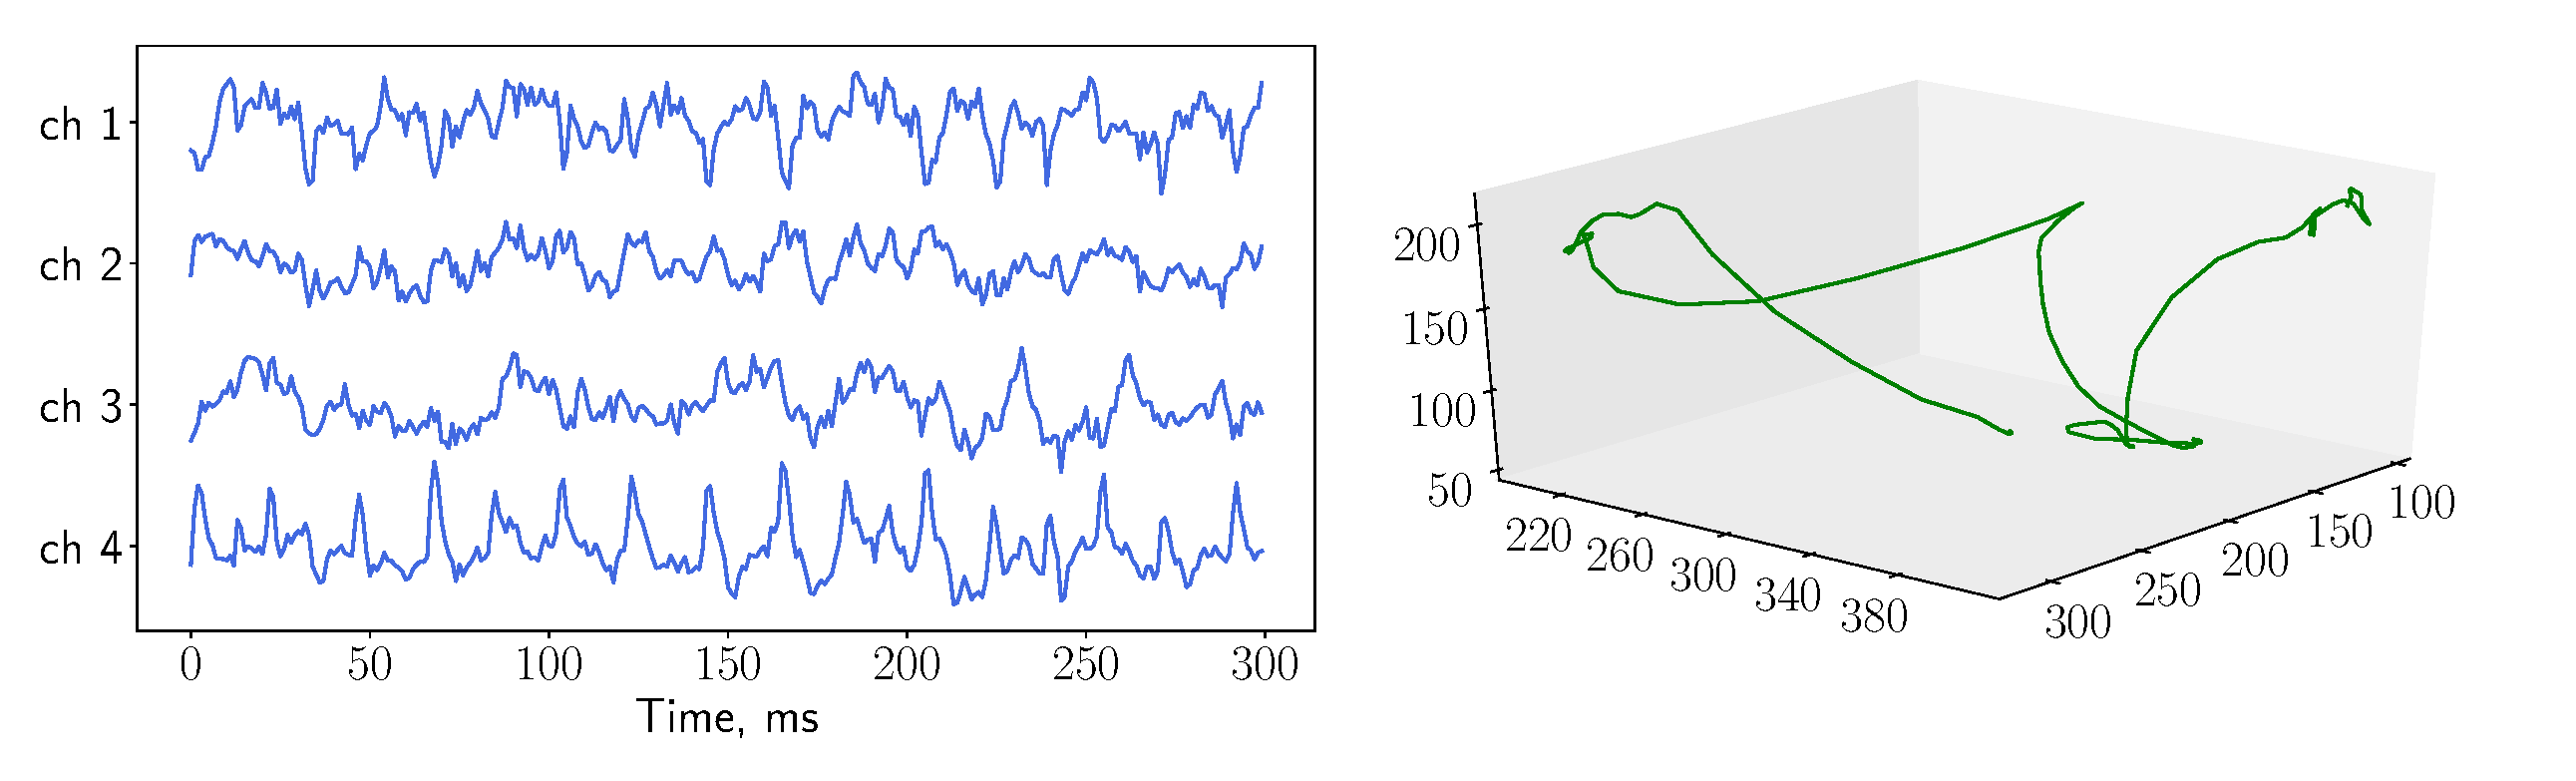
\includegraphics[width=\linewidth]{figs/ch2/ecog_data}
	\caption{Сигналы мозга (левый график) и 3D координаты руки (правый график)}
	\label{ch2:fig:ecog_data}
\end{figure}

Введём среднеквадратичную ошибку для некоторых матриц $\mathbf{A} = [a_{ij}]$ и $\mathbf{B} = [b_{ij}]$
\[
	\text{MSE} (\mathbf{A}, \mathbf{B}) = \sum_{i,j} (a_{ij} - b_{ij})^2.
\]
Для оценивания качества аппроксимации вычисляется значение нормированной среднеквадратичной ошибки
\begin{equation}
	\text{NMSE}(\bY,  \mathbf{\hat{Y}}) = \frac{\text{MSE} (\bY, \mathbf{\hat{Y}})}{\text{MSE} (\bY, \mathbf{\bar{Y}})},
	\label{ch2:eq:nmse}
\end{equation}
где $\mathbf{\hat{Y}}$~--- прогноз модели, $\mathbf{\bar{Y}}$~--- константный прогноз средним значением по столбцам матрицы.

\textbf{Результаты на данных электроэнергии.}
Для нахождения оптимальной размерности $l$ латентного пространства все данные потребления электроэнергии были разбиты на обучающую и валидационную части. 
Обучающая выборка состоит из $700$ объектов, валидационная из $370$. Зависимость нормированной квадратичной ошибки~\eqref{ch2:eq:nmse} от размерности $l$ латентного пространства представлена на Рис.~\ref{ch2:fig:energy_n_comp}. 
Сначала ошибка резко падает при увеличении размерности скрытого пространства, а затем стабилизируется.

\begin{figure}[ht]
	\centering
	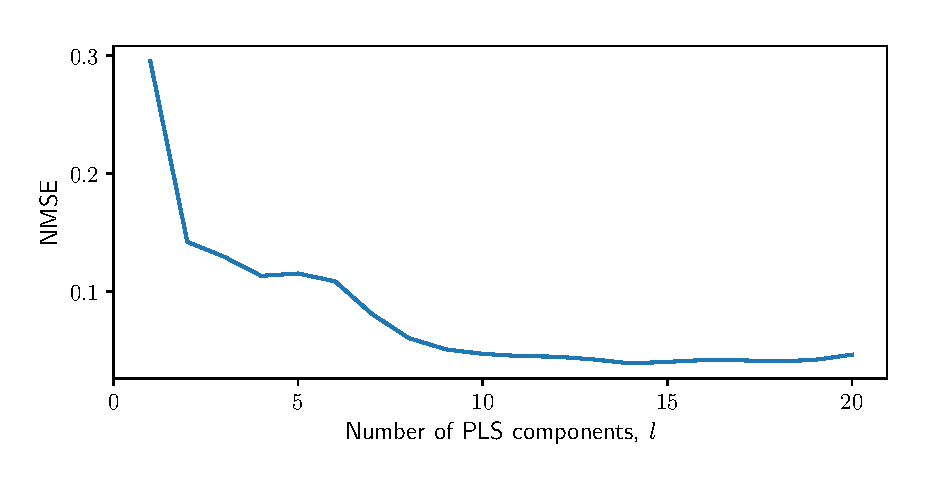
\includegraphics[width=0.75\linewidth]{figs/ch2/energy_n_comp}
	\caption{Прогноз потребления электроэнергии алгоритмом PLS при размерности латентного пространства $l$=14}
	\label{ch2:fig:energy_n_comp}
\end{figure}

Минимальная ошибка наблюдается при $l=14$. 
Построим прогноз потребления электроэнергии при данном $l$. 
Результат аппроксимации изображен на Рис.~\ref{ch2:fig:energy_prediction}. Алгоритм PLS восстановил авторегрессионную зависимость и обнаружил дневную сезонность.

\begin{figure}[ht]
	\centering
	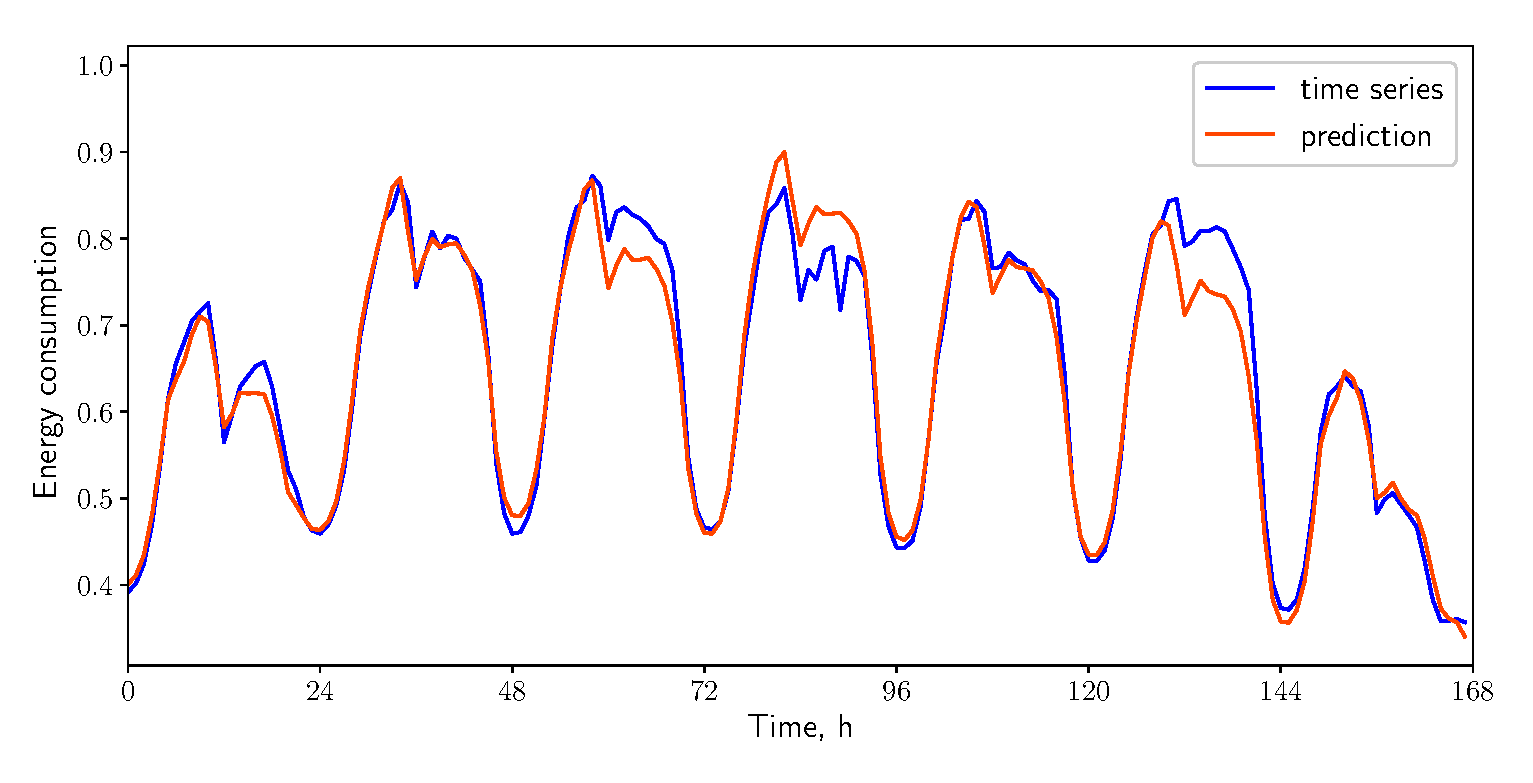
\includegraphics[width=0.95\textwidth]{figs/ch2/energy_prediction}
	\caption{Зависимость ошибки от размерности латентного пространства для данных потребления электроэнергии}
	\label{ch2:fig:energy_prediction}
\end{figure}

\textbf{Результаты на данных электрокортикограммы.}
На Рис.~\ref{ch2:fig:ecog_n_comp} представлена зависимость нормированной квадратичной ошибки~\eqref{ch2:eq:nmse} от размерности латентного пространства. Ошибка аппроксимации меняется незначительно при $l > 5$.
Таким образом совместное описание пространственно-временного спектрального представления объектов и пространственного положения руки может быть представлено вектором размерности $l \ll n$.
Зафиксируем $l = 5$. 
Пример аппроксимации положения руки изображен на Рис.~\ref{ch2:fig:ecog_prediction}. 
Сплошными линиями изображены истинные координаты руки по всем осям, пунктирными линиями показана аппроксимация методом PLS.
 
\begin{figure}[ht]
	\centering
	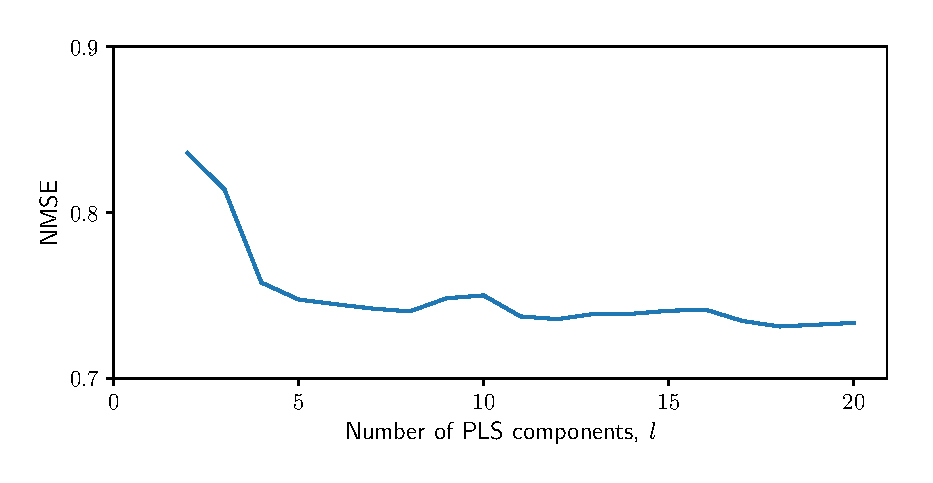
\includegraphics[width=0.75\linewidth]{figs/ch2/ecog_n_comp}	
	\caption{Зависимость ошибки от размерности латентного пространства для данных ECoG}
	\label{ch2:fig:ecog_n_comp}
\end{figure}

\begin{figure}[ht]
	\centering
	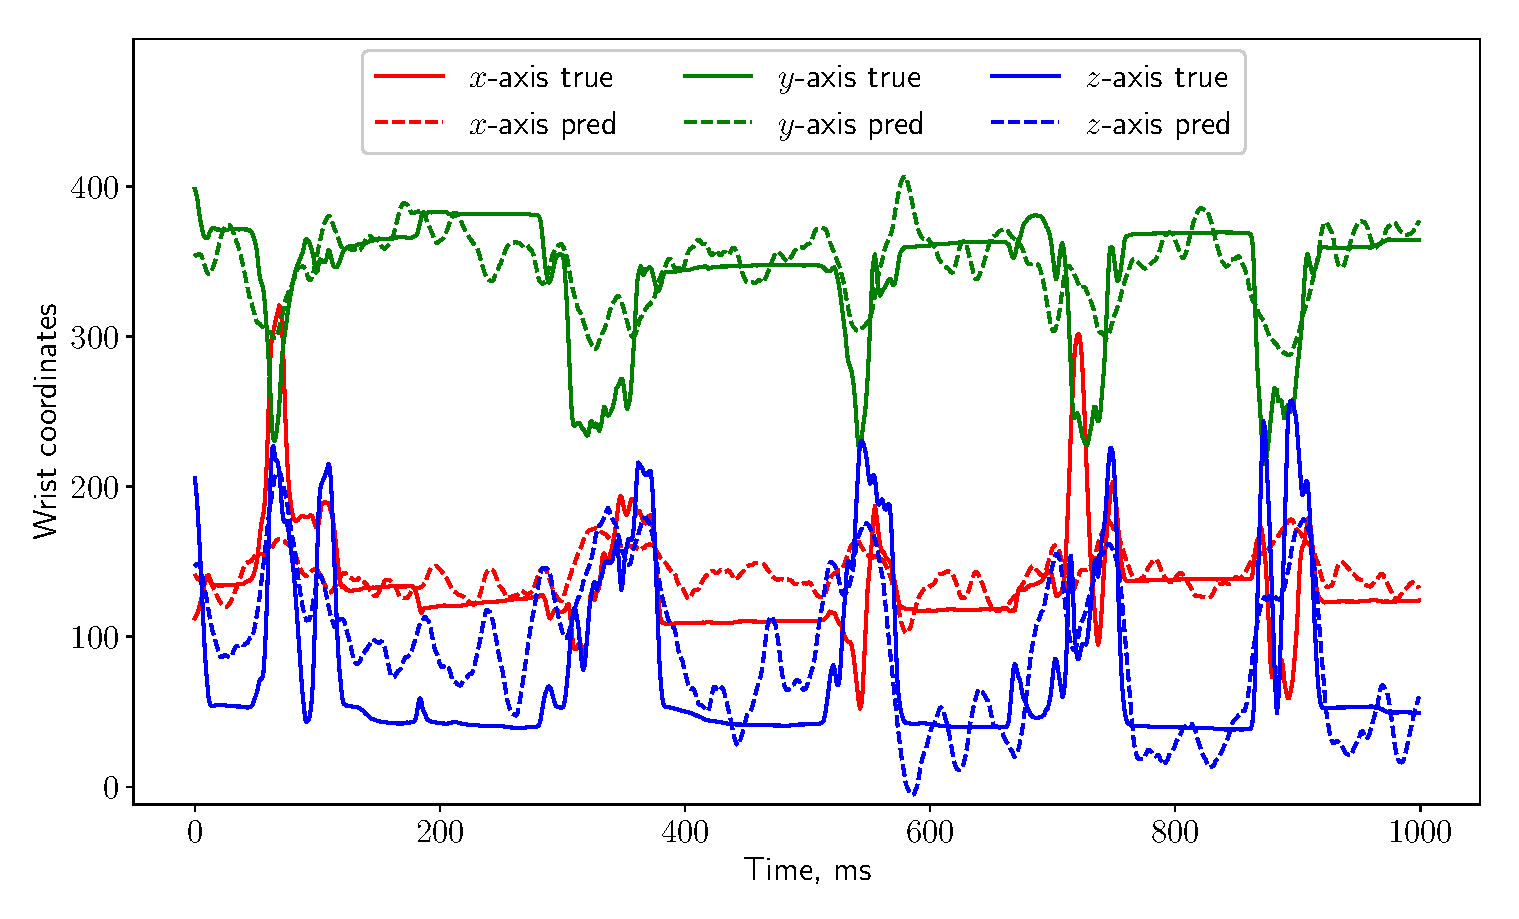
\includegraphics[width=\textwidth]{figs/ch2/ecog_prediction}
	\caption{Прогноз движения руки по данным ECoG алгоритмом PLS при размерности латентного пространства $l=5$}
	\label{ch2:fig:ecog_prediction}
\end{figure}

%%%%%%%%%%%%%%%%%%%%%%%%%%%%%%%%%%%%%%%%%%%%%%%%
\section{Анализ нелинейных зависимостей проекций в скрытое пространство}
\label{sec:ch2:exp_nonlinear}
%%%%%%%%%%%%%%%%%%%%%%%%%%%%%%%%%%%%%%%%%%%%%%%%

Цель вычислительного эксперимента~-- сравнительный анализ рассматриваемых моделей.
Рассматриваются данные, для которых сложность класса линейных методов неадекватно низка.
Нелинейные модели позволяют получить точный прогноз при адекватной сложности.

\begin{figure}[ht]
	\centering 
	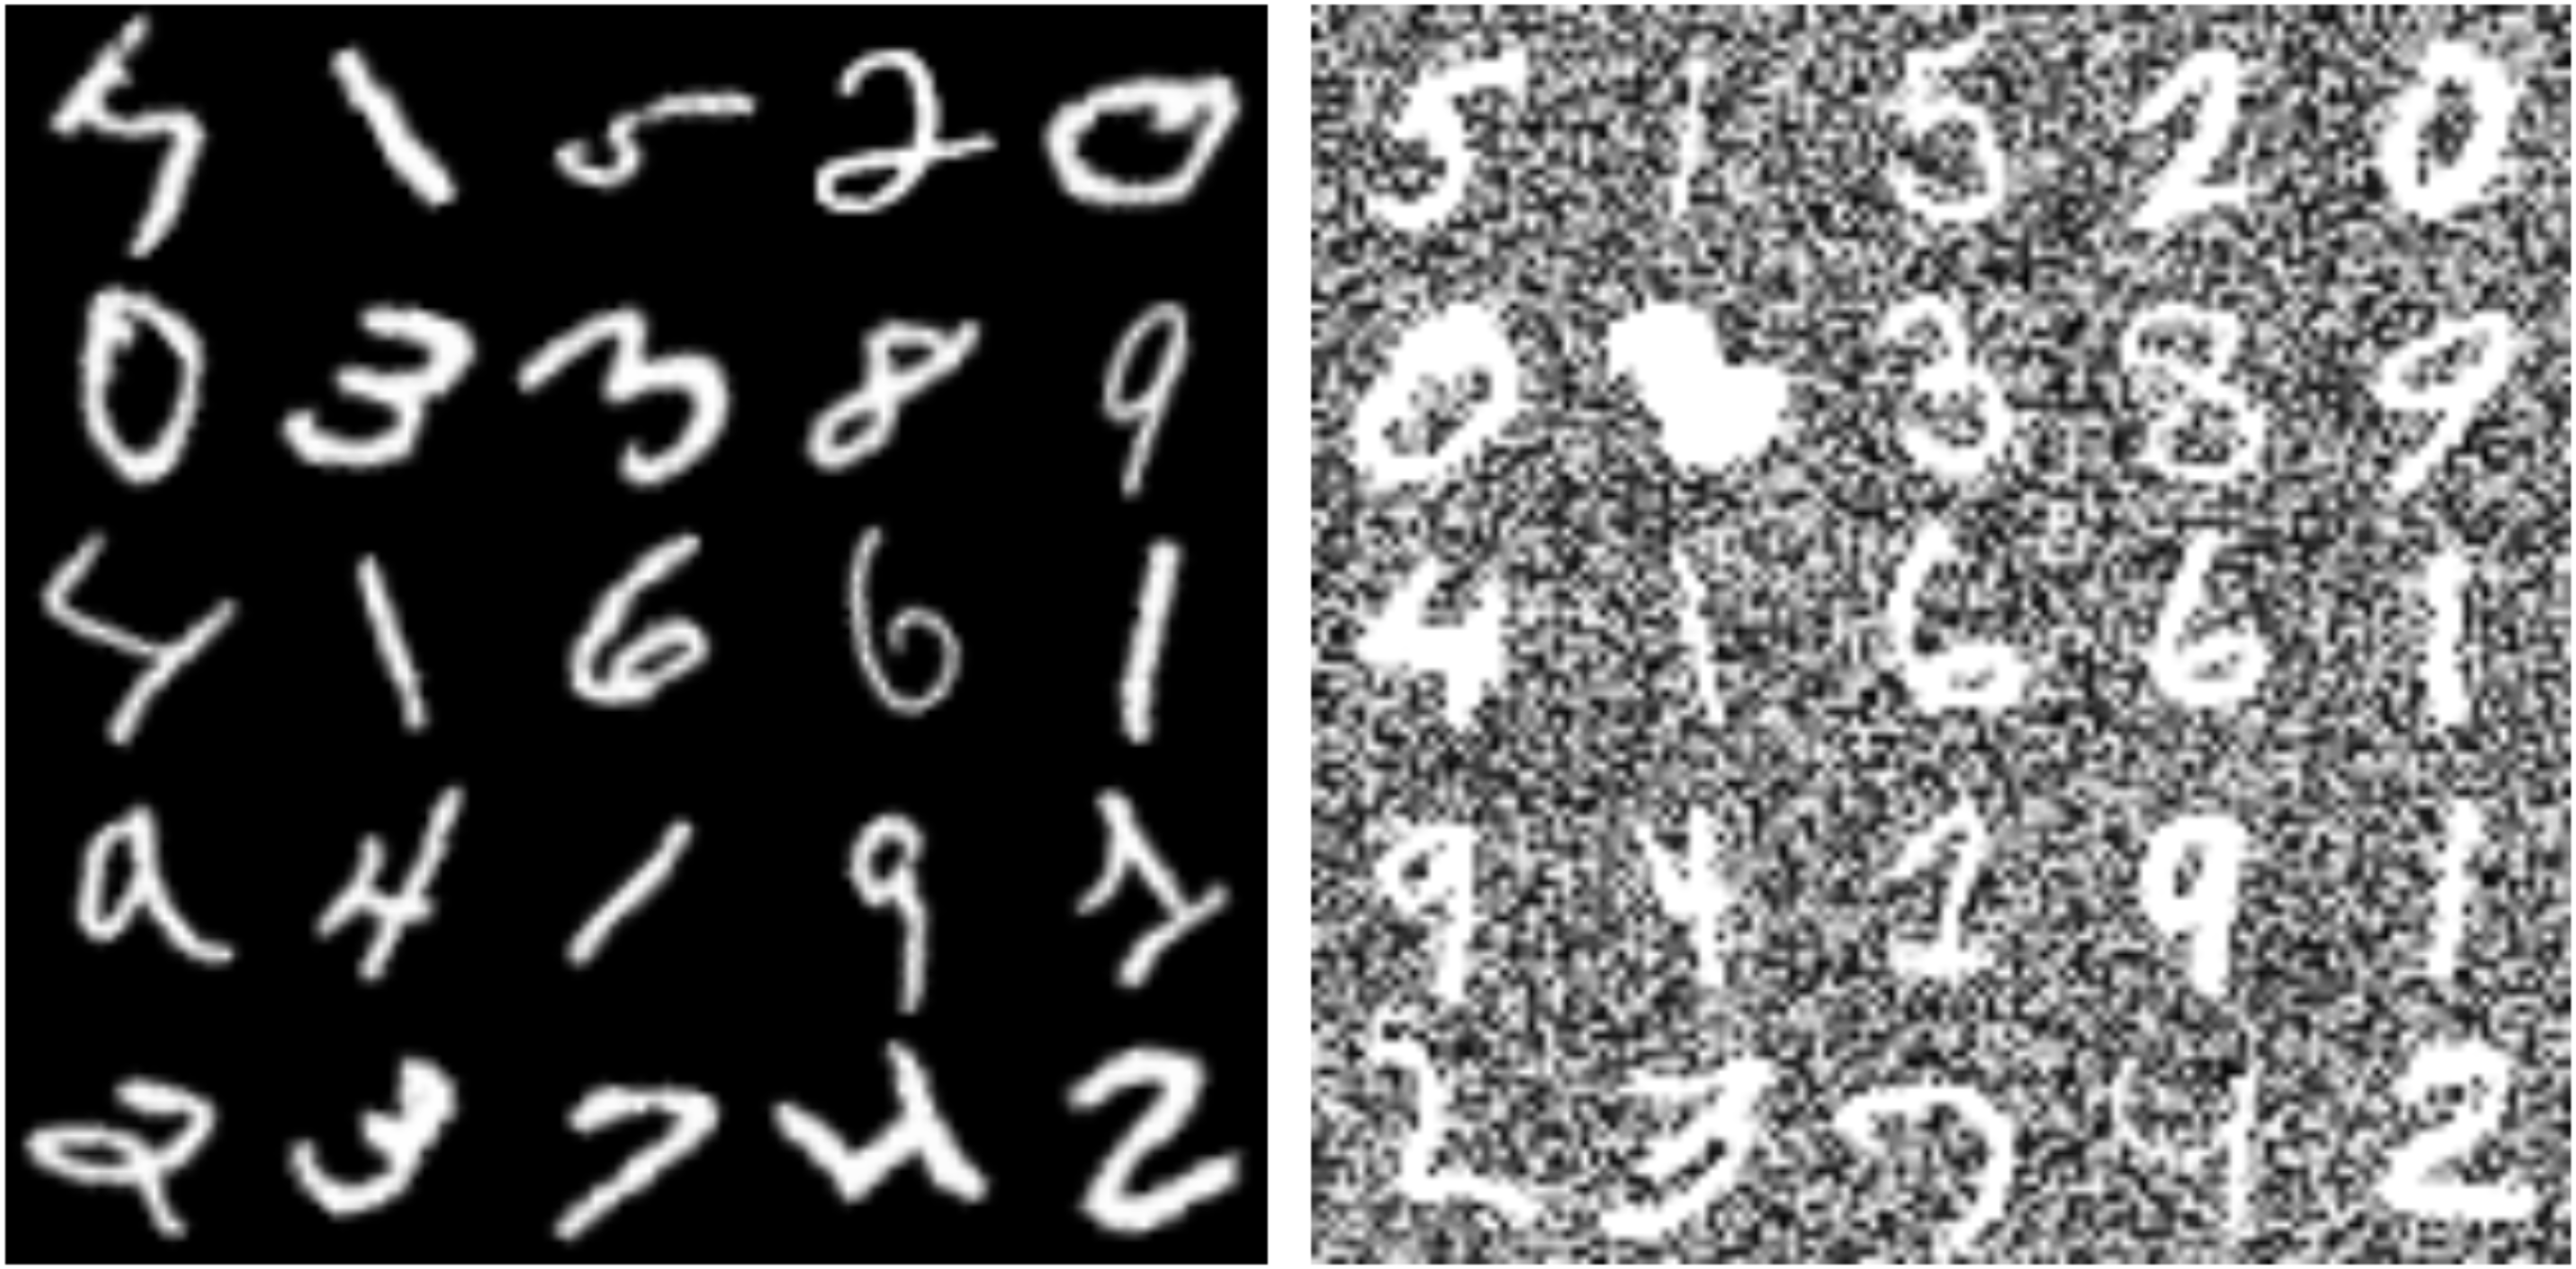
\includegraphics[width=\linewidth]{figs/ch2/noisy_mnist}
	\caption{Зашумленные изображения из набора данных MNIST}
	\label{ch2:fig:noisy_mnist}
\end{figure}

\textbf{Задача фильтрации шума.}
Проведем сравнение качества DeepCCA и CCA на задаче классификации зашумленных цифровых изображениях, представленных на Рис.~\ref{ch2:fig:noisy_mnist}. Для этого используется набор данных MNIST~\cite{MNIST}, который состоит из 70\,000 цифровых изображений $28 \times 28$ образцов рукописного написания цифр. Предлагается получить два новых набора данных $\bX$ и $\bY$ следующим образом. Первый набор получается поворотом исходных изображений на угол в диапазоне $[\frac{-\pi}{4}, \frac{\pi}{4}]$. Для получения второго набора данных для каждой картинки из первого набора данных ставится в соответствие случайным образом картинка с той же цифрой, но с добавлением независимого случайного шума, распределенного равномерно на отрезке $[0,1]$.

\begin{table}[ht]
	\caption{Точность классификации линейного SVM для алгоритмов Deep CCA и CCA}
	\centering
	\begin{tabular}{l|cc}
	\hline
		Скользящий контроль & Deep CCA ($L=3$) & CCA \\  \hline
		Валидация & 92,74\%  &  76,21\%\\
		Тест & 92,14\% & 76,07\% \\
		\hline
	\end{tabular}
	\label{ch2:tbl:svm_cca}
\end{table}

Применив к двум новым наборам данных DeepCCA или CCA, получаем новое низкоразмерное признаковое пространство, которое игнорирует шумы в исходных данных. Модель DeepCCA представляет собой нейронную сеть с $L=3$ скрытыми слоями. Таким образом, получаем функции кодирования $\bphi_e$ и $\bpsi_e$ для исходных наборов данных. На новых признаках, полученных разными моделями (DeepCCA и CCA), для первого набора данных, то есть на данных после применения функции кодирования $\bphi_e$ к первому набору исходных данных, обучим линейный SVM-классификатор. Показателем эффективности будет точность классификации линейного SVM на тестовых данных. В случае построения адекватного скрытого пространства полученные образы объектов будут линейно разделимы. Результаты эксперимента приведены в таблице~\ref{ch2:tbl:svm_cca}. Точность классификации нелинейной модели существенно выше линейного алгоритма CCA.

\textbf{Задача восстановления изображений.}
Для анализа процедуры согласования проведен вычислительный эксперимент с предложенными нелинейными моделями.
Для снижения размерности пространства используются нейросетевые модели автоэнкодера c согласованием скрытого пространства~\eqref{ch2:eq:concordance}.
В качестве базовых моделей используются модель автоэнкодера без согласования скрытых пространств, а также линейный PLS. В качестве исходного набора данных используется набор данных MNIST~\cite{MNIST}. Каждое изображение поделено на левую и правую части, как показано на Рис.~\ref{ch2:fig:left_right_mnist}. Модель по левому изображению восстанавливает правое изображение.

\begin{figure}[ht]
\centering 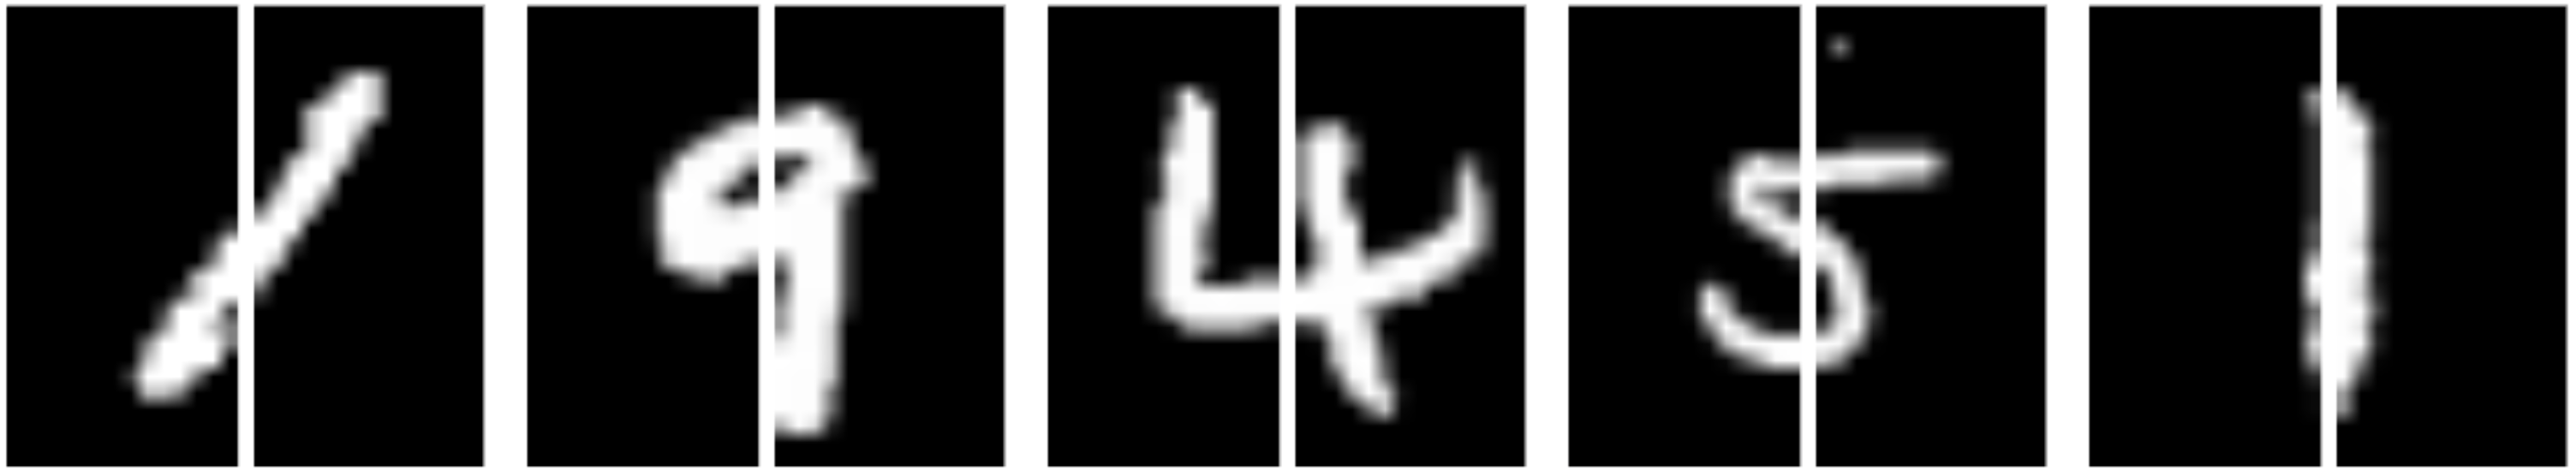
\includegraphics[width=\linewidth]{figs/ch2/left_right_mnist}
\caption{Набор данных MNIST, в котором каждое изображение разделено пополам}
\label{ch2:fig:left_right_mnist}
\end{figure}

Модель EncNet1~--- нейронная сеть с нелинейными функциями активации, которая обучается на данных после преобразования их автоэнкодером. Модель LinNet1~--- нейронная сеть с одним линейным слоем, которая также обучается на преобразованных данных. Для EncNet1 и LinNet1 автоэнкодеры для исходных и целевых объектов используют совместную функцию потерь, которая связывает выходы энкодеров. Модели EncNet2 и LinNet2 устроены аналогично EncNet1 и LinNet1 соответственно, но в автоэнкодерах нет совместной функции потерь. Модель DumbNet~---  нейронная сеть, которая обучается на исходных данных и имеет такую же структуру, что и EncNet, то есть имеет такое же число слоев и в каждом слое такое же количество нейронов, что и у EncNet.

Для оценки качества моделей вычислялась среднеквадратичная ошибка. Примеры восстановленных изображений показаны на Рис.~\ref{ch2:fig:mnist_nn_preds}. Качество моделей, а также их сложность представлены в таблице~\ref{ch2:tbl:mnist_nn_error}.
На Рис.~\ref{ch2:fig:mnist_nn_preds} показано, что предложенные модели EncNet и LinNet позволяют получить более четкие и различимые изображения, в отличие от базовой нелинейной модели DumbNet и линейной модели PLS.
Несмотря на заметное улучшение визуального качества изображений, ошибка предложенных моделей выше, чем у модели DumbNet.
Это связано с тем, что среднеквадратичная ошибка оказалась неадекватной метрикой в пространстве изображений.
Нахождение оптимальной метрики для оценки качества предложенных алгоритмов может быть одним из возможных направлений развития текущего эксперимента.

\begin{table}[!ht]
	\caption{Квадратичная ошибка для нелинейных моделей в задаче восстановления правой части изображения по левой}
	\centering
	\small
	\begin{tabular}{l|cccccc}
	\hline
		& EncNet1 & LinNet1 & EncNet2 & LinNet2 & DumbNet & PLS\\  \hline
		Число параметров, тыс. & 283 & 239 & 283 & 239  & 283 & --\\
		Ошибка на тесте & 0,147 & 0,235 & 0,149 & 0,236 & 0,128 & 0,188 \\
		\hline
	\end{tabular}
	\label{ch2:tbl:mnist_nn_error}
\end{table}

\begin{figure}[!ht]
	\centering 
	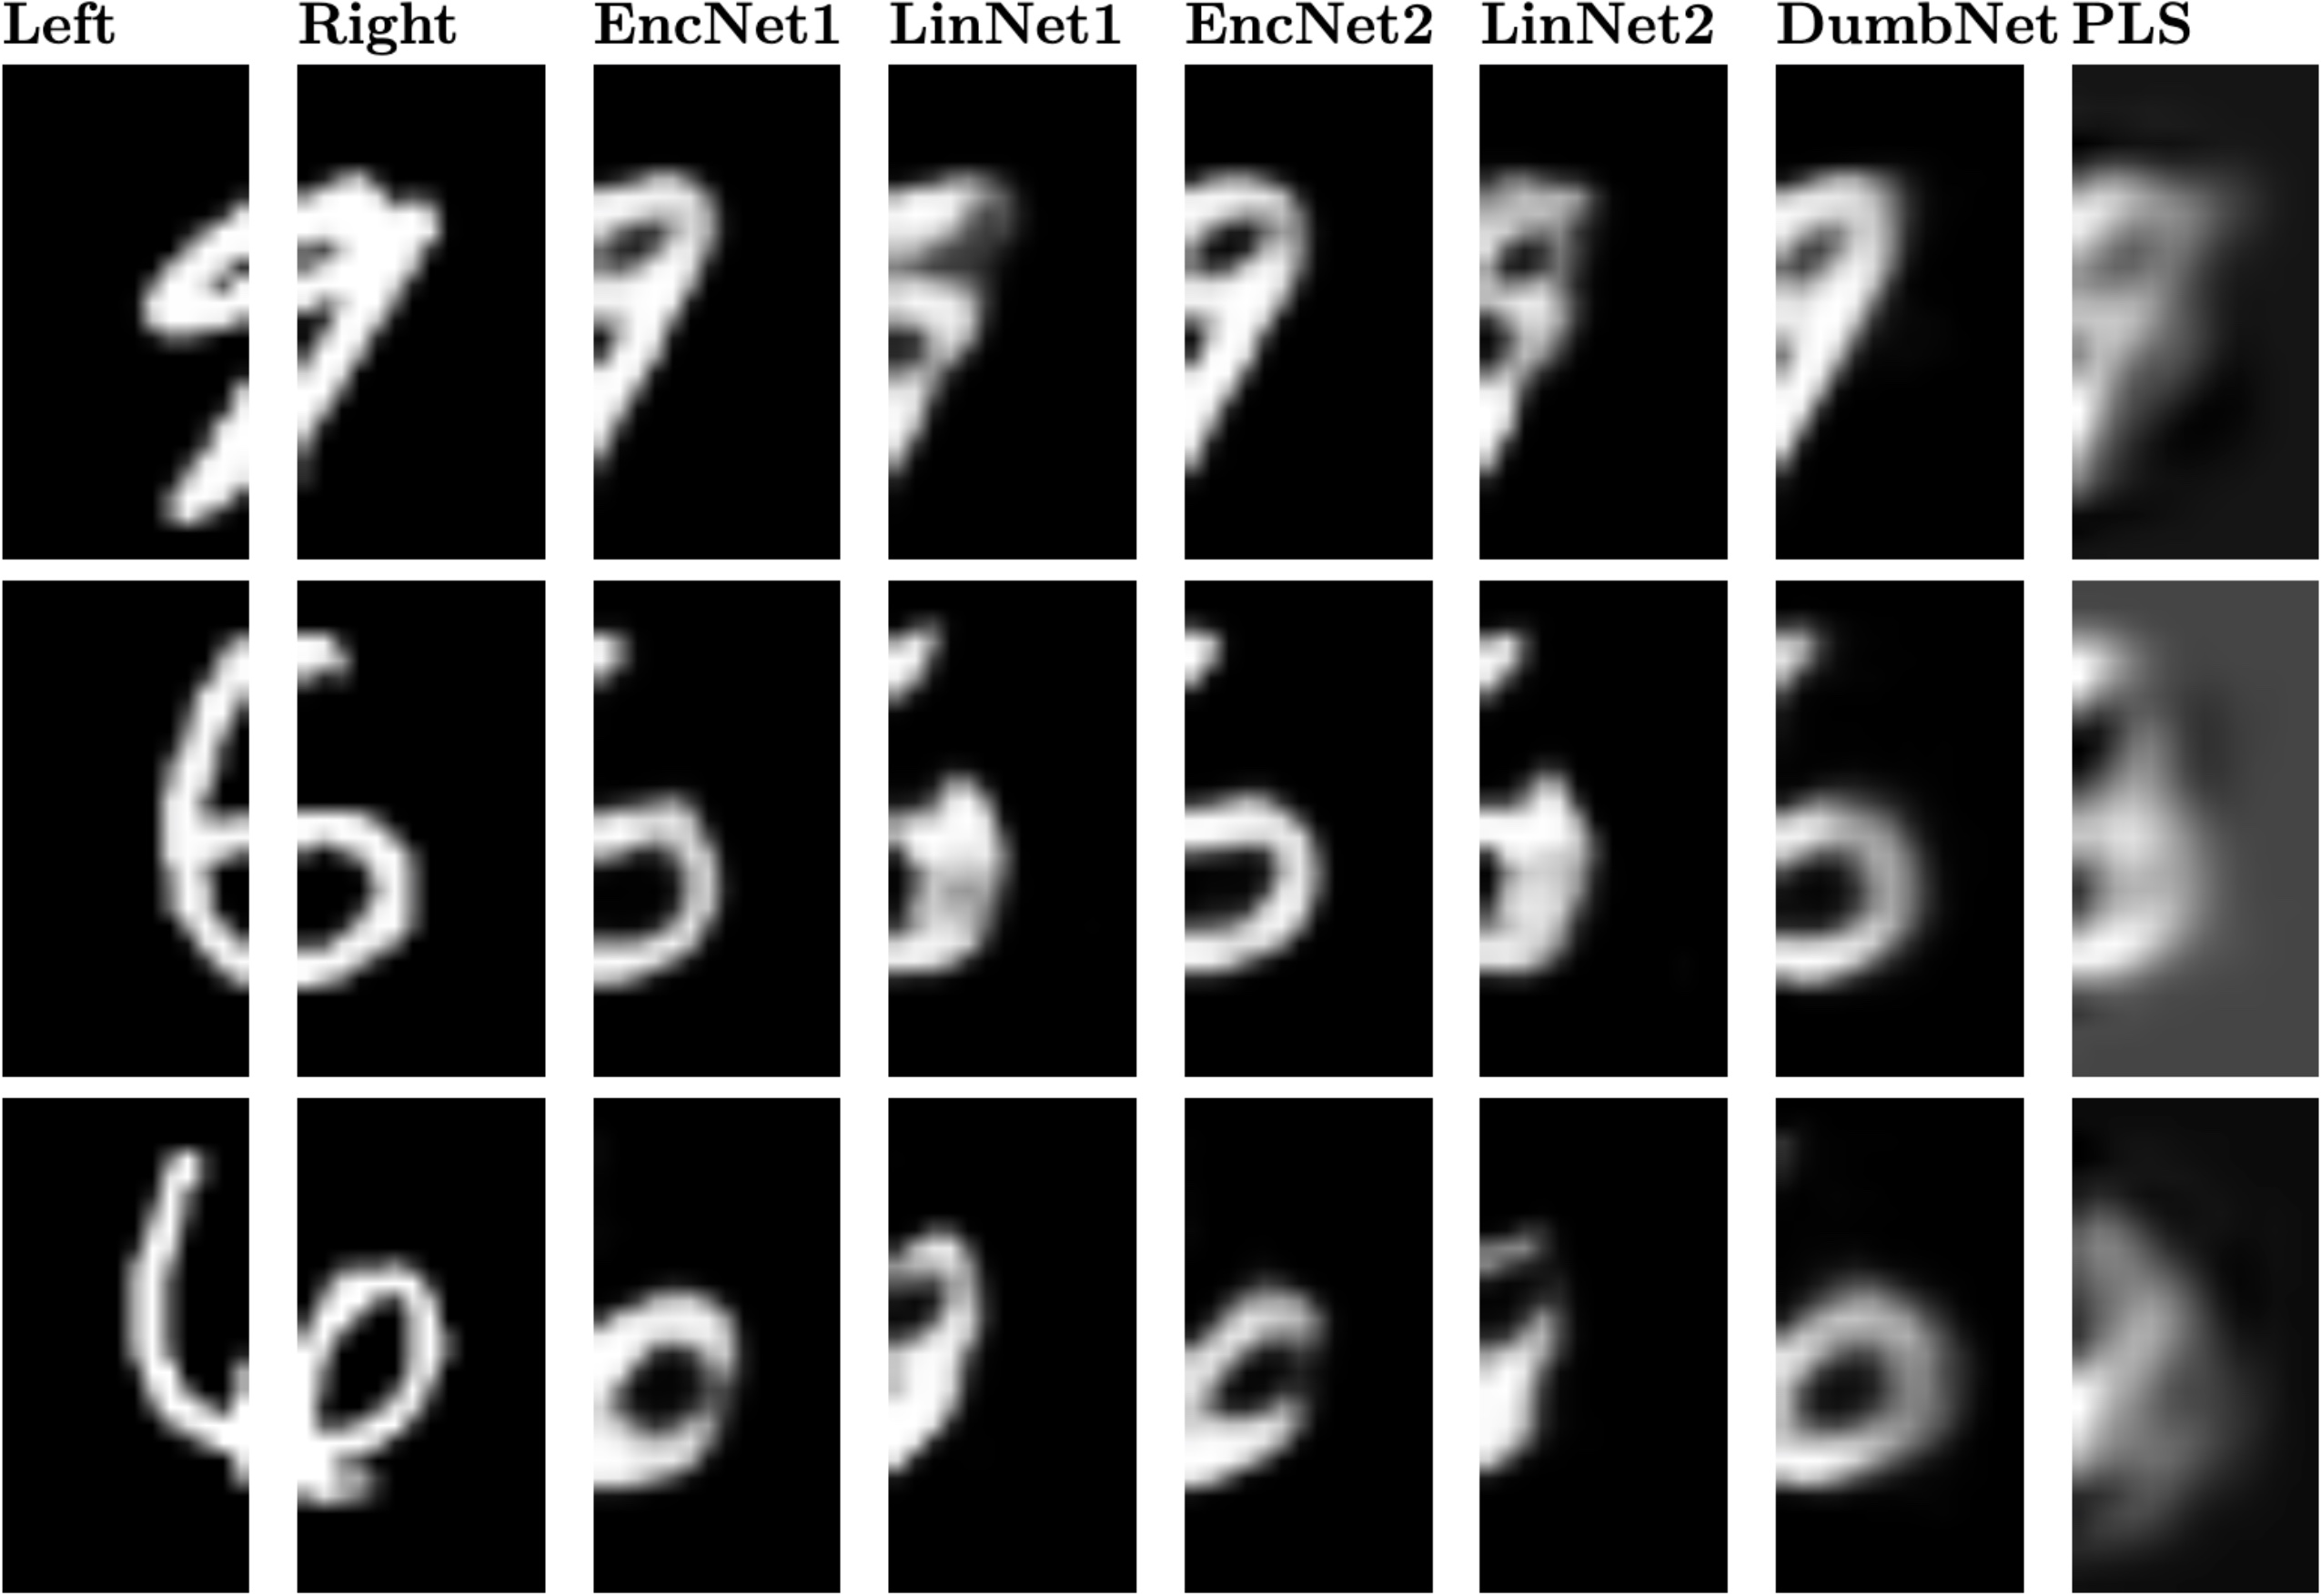
\includegraphics[width=\linewidth]{figs/ch2/mnist_preds}
	\caption{Пример реконструкции правой части изображения по левой для рассматриваемых моделей}
	\label{ch2:fig:mnist_nn_preds}
\end{figure}
